\documentclass[12pt,a4paper,ngerman]{article}
\usepackage{stylesheet}
\begin{document}
\TUHeader                          %  Bitte Ausfüllen!!!
%----------------------------
{Übung F: Übertragungsverhalten nachrichtentechnischer Systeme}                       %  Übungstitel
%----------------------------
{25.11.2014}                        %  Übungsdatum
%----------------------------
{05}                            %  Gruppen-Nr.
%----------------------------
{Thomas Neff}                   % Name des Protokollführers
%----------------------------
{
1.~Daniel Freßl, 1230028\\
2.~Thomas Neff, 1230319\\                    %  Übungsteilnehmer
3.~Thomas Pichler, 1230320 \\                   %  ...bei <4 Teilnehmer auskommentieren
4.~Martin Winter, 1130688\\
5.~Bernadette Schreyer, 1073076\\
}
%----------------------------
{Ao.Univ.-Prof. Dipl.-Ing. Dr. techn. Erich Leitgeb}
{Max Henkel}                          %  Betreuer
%----------------------------
{Graz}                              %  Ort der Protokollerstellung
{\today}                            %  Datum Protokollerstellung




\pagebreak
  
\tableofcontents
  
\pagebreak

%-------------------------------------------------------------------------------
%
% Beginn des Protokolls
%
%-------------------------------------------------------------------------------

\section{Rückwirkungsfreie Messung des H-Feldes zweier PCD-Schleifenantennen mit unterschiedlichen Güten}
\subsection{Aufgabenstellung}
Der Zweck dieser Übung besteht darin, Energie- und Informatuonsübertragung (Von Lesegerät zu Transponder-Karte) für RFID-Systeme in Abhängigkeit der Güte der PCD-Sendeantenne deutlich zu machen. Bei gleicher Treiberleitsung kann man mit einer höheren Antennengüte eine höhere H-Feldstärke erreichen, verliert jedoch in der zeitlichen Auflösung von Pulsen, dies bedeutet eine geringere mögliche Datenrate. 
\begin{itemize}
\item Nehmen Sie hierfür bei zwei Antennen, unterschiedlicher Güte, die Feldstärke in Abhängigkeit der Distanz auf.
\item Nehmen Sie die Anstiegszeiten bei beiden Antennen auf.
\end{itemize}
%\cite[18]{skript}

\subsection{Messaufbau}

\subsection{Tabellen}

\centering
\begin{tabular}{ |c|c|c|c|c| }
  \hline
     & Q=50 & Q=5 & Q=50 & Q=5\\

    Distanz & $U_i(pp)$ & $U_i(pp)$ & H(rms) & H(rms)\\

  [mm] & [V] & [V] & [A/m] & [A/m] \\
  \hline
  0 & $2.9$ & $0.894$ & & \\
  \hline
  $0.5$ & $2.75$ & $0.863$ & & \\
  \hline
  $1$ & $2.61$ & $0.813$ & & \\
  \hline
  $1.5$ & $2.44$ & $0.756$ & & \\
    \hline
  $2$ & $2.25$ & $0.706$ & & \\
    \hline
  $2.5$ & $2.06$ & $0.637$ & & \\
    \hline
  $3$ & $1.89$ & $0.584$ & & \\
    \hline
  $3.5$ & $1.7$ & $0.531$ & & \\
    \hline
  $4$ & $1.55$ & $0.481$ & & \\
    \hline
  $4.5$ & $1.39$ & $0.434$ & & \\
    \hline
  $5$ & $1.25$ & $0.425$ & & \\
    \hline
  $5.5$ & $1.13$ & $0.425$ & & \\
     \hline
  $6$ & $1.01$ & $0.425$ & & \\
      \hline
  $6.5$ & $0.92$ & $0.425$ & & \\ 
      \hline
  $7$ & $0.82$ & $0.425$ & & \\
      \hline
  $7.5$ & $0.75$ & $0.425$ & & \\
      \hline
  $8$ & $0.68$ & $0.425$ & & \\
      \hline
  $8.5$ & $0.62$ & $0.425$ & & \\
      \hline
  $9$ & $0.55$ & $0.425$ & & \\
      \hline
  $9.5$ & $0.5$ & $0.425$ & & \\
      \hline
  $10$ & $0.46$ & $0.425$ & & \\
      \hline
  $10.5$ & $0.41$ & $0.425$ & & \\
      \hline
  $11$ & $0.38$ & $0.425$ & & \\
      \hline
  $11.5$ & $0.35$ & $0.425$ & & \\
      \hline
  $12$ & $0.32$ & $0.425$ & & \\
      \hline
  $12.5$ & $0.29$ & $0.425$ & & \\
      \hline
  $13$ & $0.29$ & $0.425$ & & \\
      \hline
  $13.5$ & $0.29$ & $0.425$ & & \\
        \hline
  $14$ & $0.29$ & $0.425$ & & \\
  \hline
 
\end{tabular}

\subsection{Formeln}

\begin{equation}
U_{ind} = 2 \cdot  \pi \cdot f_r \cdot \mu_e \cdot \mu_r \cdot H \cdot A
\end{equation}

\begin{equation}
U_{SS} = \sqrt{2}  \cdot 2 \cdot U_{ind}
\end{equation}
\pagebreak
\subsection{Berechnungsbeispiele}

\begin{equation}
U_{ind} = 2 \cdot  \pi \cdot f_r \cdot \mu_e \cdot \mu_r \cdot H \cdot A
\end{equation}

\begin{equation}
U_{SS} = \sqrt{2}  \cdot 2 \cdot U_{ind}
\end{equation}

\subsection{Diagramme}
%\begin{figure}[H]
%\centering
%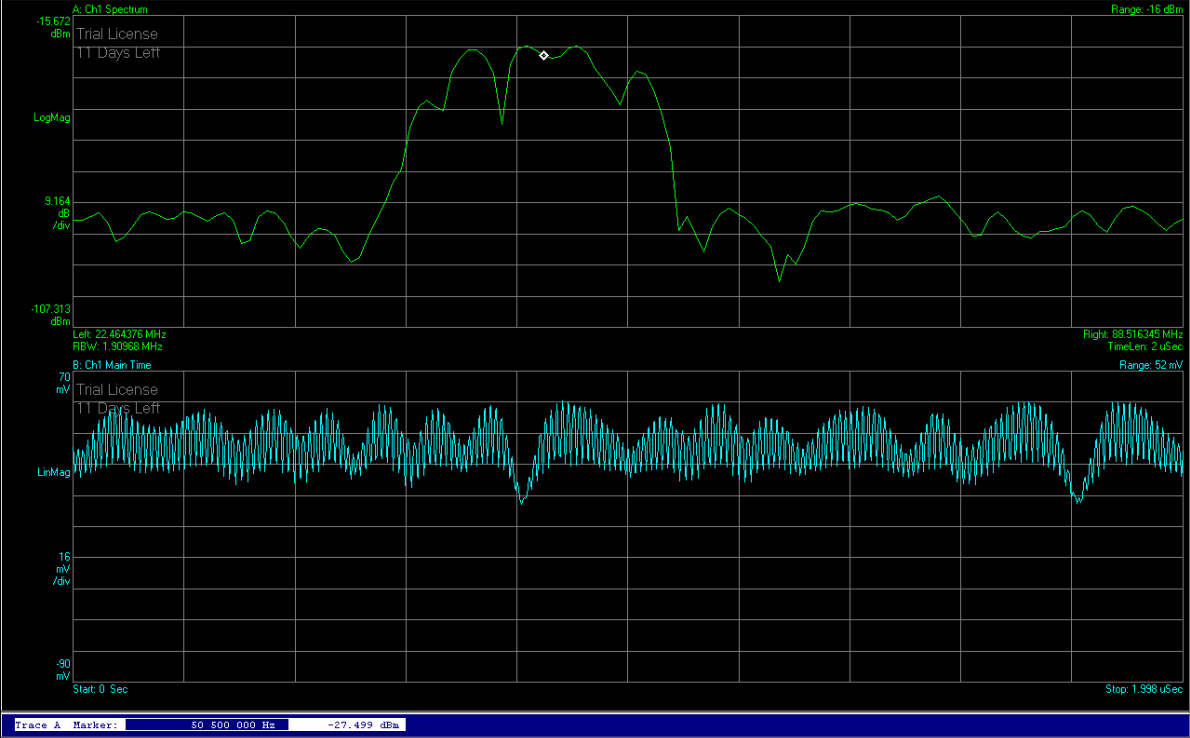
\includegraphics[width=0.9\textwidth]{figures/Aufgabe1_QPSK.jpg} 
%\caption{Signal in Frequenz- und Zeitbereich}
%\label{fig:1_sig}
%\end{figure}


\subsection{Diskussion}


\pagebreak



\section{Messung der H-Feldstärke über der Frequenz bei unterschiedlichen Antennengüten}
\subsection{Aufgabenstellung}
Der Zweck dieser Übung besteht darin, die starke Frequenzabhängigkeit bei Antennen hoher Güte (Bandpass-Filter) im Frequenzbereich zu zeigen. Hochgütige Antennen haben eine starke Resonanzerhöhung an der Resonanzfrequenz, niedergütige Antennen einen eher flachen Verlauf. Bei Frequenzen deutlich über oder unter der Resonanzfrequenz, im Fall von RFID-Systemen insbesondere den Unterträgern, welche die Transponderkarten zur Rückmodulation nutzen , können hochgütige Antennen durchaus eine deutlich größere Dämpfung haben, als niedergütige Sendeantennen. Dies hat Einfluss auf die Empfindlichkeit im Empfangszweig eines Lesegerätes.
\begin{itemize}
\item Messen Sie die Frequenzabhängigkeit zweier Antennen mit unterschiedlciher Güte und stellen Sie den Verlauf grafisch dar.
\end{itemize}


\subsection{Messaufbau}

\subsection{Tabellen}
\centering
\begin{tabular}{ |c|c|c|c|c| }
  \hline
     & Q=50 & Q=5 & Q=50 & Q=5\\

    Frequenz & $U_i(pp)$ & $U_i(pp)$ & H(rms) & H(rms)\\

  [MHz] & [V] & [V] & [A/m] & [A/m] \\
  \hline
  12 & $0.363$ & $0.5$ & & \\
  \hline
  $12.2$ & $0.425$ & $0.575$ & & \\
  \hline
  $12.4$ & $0.5$ & $0.547$ & & \\
  \hline
  $12.6$ & $0.784$ & $0.813$ & & \\
    \hline
  $12.8$ & $1$ & $0.844$ & & \\
    \hline
  $13$ & $1.3$ & $0.869$ & & \\
    \hline
  $13.2$ & $1.78$ & $0.887$ & & \\
     \hline
  $13.25$ & $1.97$ & $0.894$ & & \\ 
    \hline
  $13.3$ & $2.14$ & $0.9$ & & \\
    \hline
  $13.35$ & $2.31$ & $0.906$ & & \\
    \hline
  $13.4$ & $2.5$ & $0.906$ & & \\
    \hline
  $13.45$ & $2.64$ & $0.906$ & & \\
    \hline
  $13.5$ & $2.73$ & $0.913$ & & \\
     \hline
  $13.55$ & $2.76$ & $0.913$ & & \\
      \hline
  $13.6$ & $2.7$ & $0.913$ & & \\ 
      \hline
  $13.65$ & $2.61$ & $0.919$ & & \\
      \hline
  $13.7$ & $2.45$ & $0.925$ & & \\
      \hline
  $13.75$ & $2.31$ & $0.925$ & & \\
      \hline
  $13.8$ & $2.14$ & $0.925$ & & \\
      \hline
  $14$ & $1.59$ & $0.925$ & & \\
      \hline
  $14.2$ & $1.23$ & $0.925$ & & \\
      \hline
  $14.4$ & $1.02$ & $0.919$ & & \\
      \hline
  $14.6$ & $0.86$ & $0.906$ & & \\
      \hline
  $14.8$ & $0.734$ & $0.9$ & & \\
      \hline
  $15$ & $0.653$ & $0.887$ & & \\
      \hline
  \hline
 
\end{tabular}
\subsection{Formeln}

\subsection{Berechnungsbeispiele}


\pagebreak
\subsection{Diagramme}
%\begin{figure}[H]
%\centering
%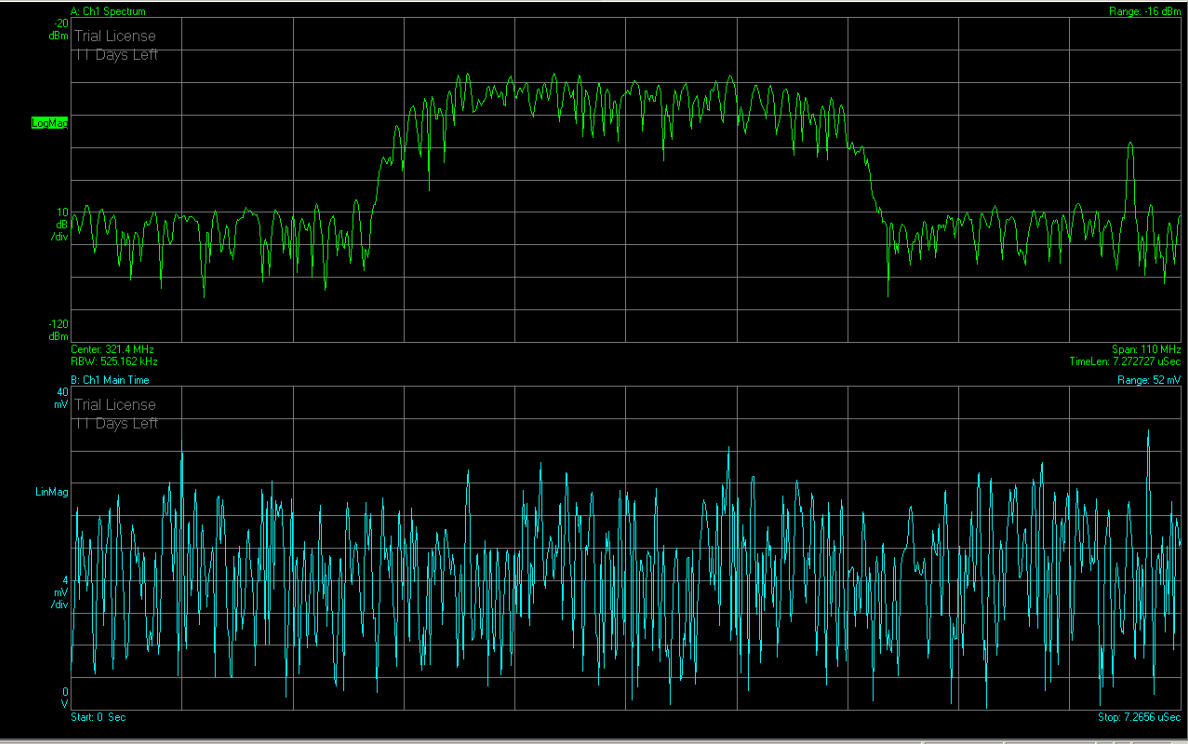
\includegraphics[width=0.9\textwidth]{figures/Aufgabe2_16QAM_1.jpg} 
%\caption{Spektrum und zeitlicher Verlauf des empfangenen 16-QAM modulierten Signals}\label{fig:aufg2_16QAM_spec}
%\end{figure}


\subsection{Diskussion}

\pagebreak



\section{Arbeitsbereich eines Lesegerätes}
\subsection{Aufgabenstellung}

\begin{itemize}
\item ???.
\end{itemize}


\subsection{Tabellen}
\begin{tabular}{ |c|c|c| }
  \hline

    H(rms)) & $U_i(pp) am Scope$ & $U_i(pp) am Transponder$\\

	[A/m] & [V] & [V] \\
  \hline
  0 & $0$ & $0$\\
  \hline
  $0.5$ & $0.456$ & $0.982$ \\
  \hline
  $1$ & $0.913$ & $1.933$\\
  \hline
  $1.5$ & $1.344$ & $3.154$\\
    \hline
  $2$ & $1.8$ & $4.21$\\
    \hline
  $2.5$ & $2.23$ & $5.26$ \\
    \hline
  $3$ & $2.69$ & $6.29$\\
     \hline
  $3.5$ & $3.19$ & $7.46$ \\ 
    \hline
  $4$ & $3.61$ & $8.5$  \\
    \hline
  $4.5$ & $4.09$ & $9.5$  \\
    \hline
  $5$ & $4.59$ & $10.52$  \\
    \hline
  $5.5$ & $5.03$ & $11.55$  \\
    \hline
  $6$ & $5.47$ & $12.55$ \\
     \hline
  $6.5$ & $5.91$ & $13.53$ \\
      \hline
  $7$ & $6.34$ & $14.55$ \\ 
      \hline
  $7.5$ & $6.78$ & $15.56$  \\
      \hline
  $8$ & $7.19$ & $16.5$  \\
      \hline
  \hline
 
\end{tabular} 
\subsection{Formeln}

\subsection{Berechnungsbeispiele}


\pagebreak
%\subsection{Diagramme}
%\begin{figure}[H]
%\centering
%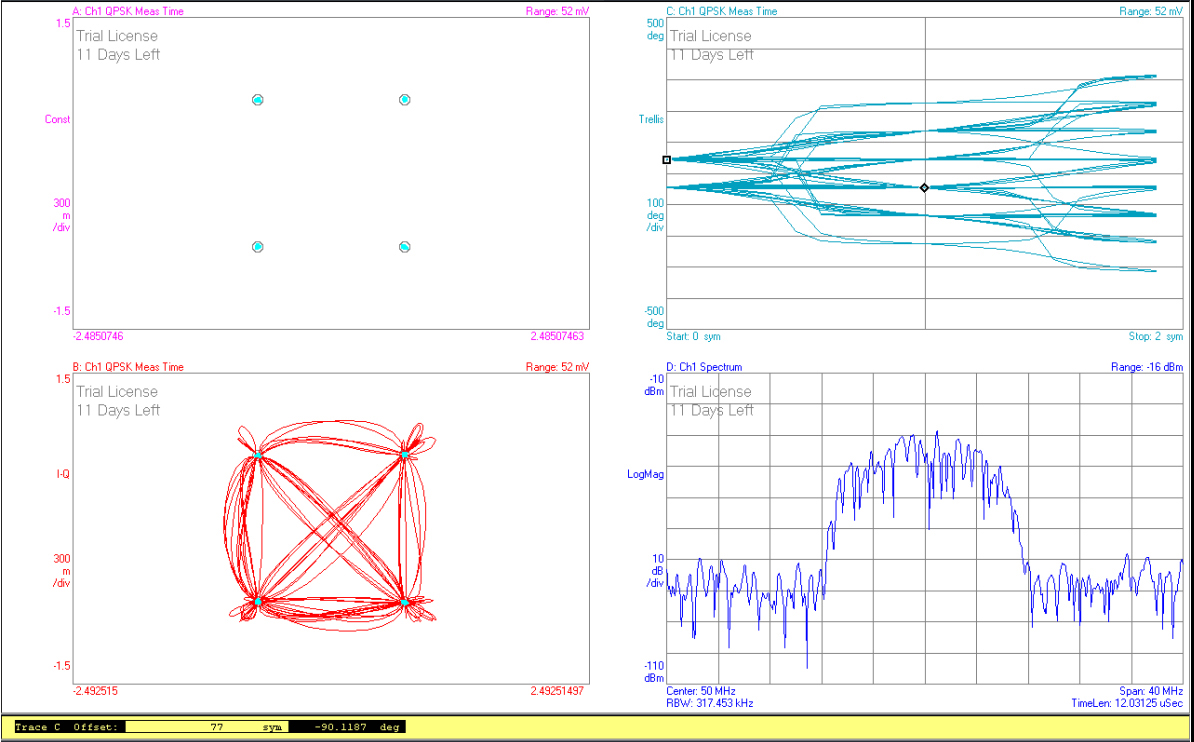
\includegraphics[width=0.9\textwidth]{figures/Aufgabe3_QPSK.jpg} 
%\caption{Konstellationsdiagramm, Phasenverlauf, Spektrum eines QPSK modulierten Signals}
%\label{fig:3_QPSK}
%\end{figure}

\subsection{Diskussion}

\section{Seitenbandpegel der Rückmodulation}
\subsection{Aufgabenstellung}

\begin{itemize}
\item???.
\end{itemize}


\subsection{Messaufbau}

\subsection{Tabellen}
\begin{tabular}{ |c|c|c| }
  \hline

    H(rms)) & $U_i(pp) oberes Seitenband$ & $U_i(pp) unteres Seitenband$\\

	[A/m] & [mV] & [mV] \\
  \hline
  1 & $320.6$ & $41.95$\\
  \hline
  $2$ & $866.21$ & $727.24$ \\
  \hline
  $3$ & $158.54$ & $32.35$\\
  \hline
  $4$ & $218.7$ & $312.14$\\
    \hline
  $5$ & $175.37$ & $61.54$\\
    \hline
  $6$ & $323.9$ & $267.93$ \\
    \hline
  \hline
 
\end{tabular} 
\subsection{Formeln}

\subsection{Berechnungsbeispiele}

\subsection{Diagramme}
%\begin{figure}[H]
%\centering
%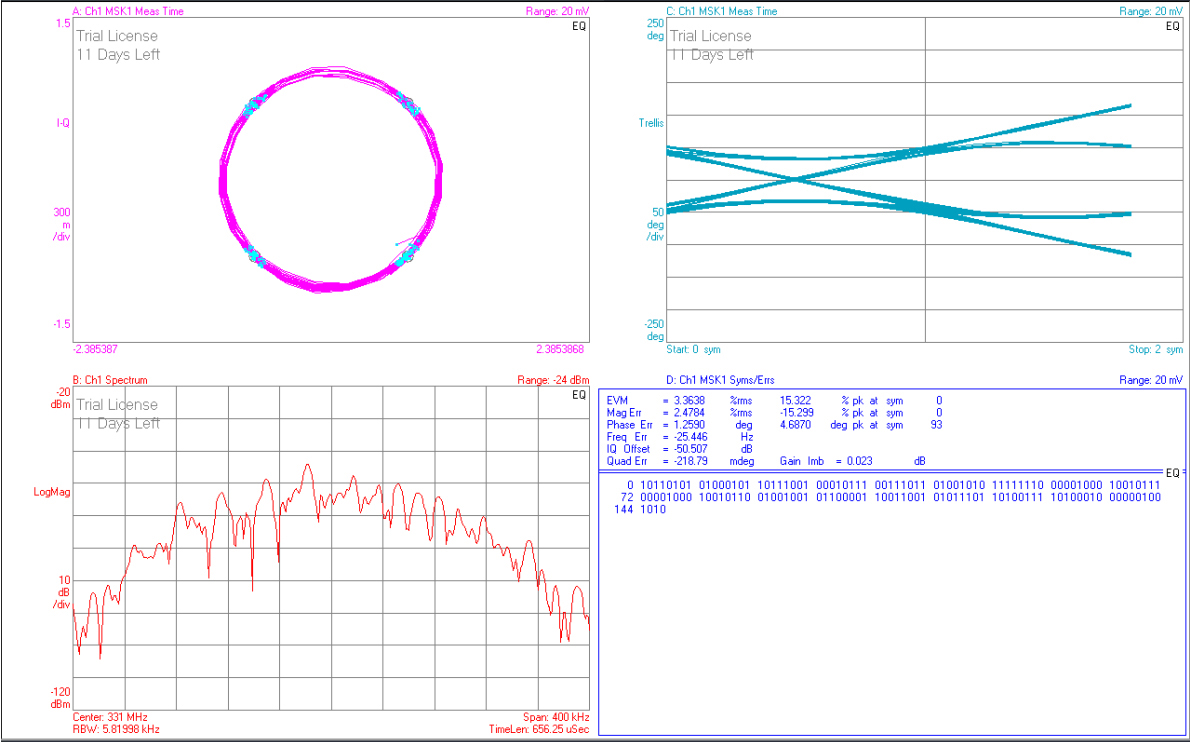
\includegraphics[width=0.9\textwidth]{figures/Aufgabe4_demod.jpg} 
%\caption{Konstellationsdiagramm, Trellis-Eye, Spektrum, Kennwerte des demodulierten GSM-Signals}
%\label{fig:a4demod}
%\end{figure}

\subsection{Diskussion}

\begin{thebibliography}{9}

\bibitem{skript}
  Markus Lenzhofer, Paul Meissner, Dr. Klaus Witrisal.
  \emph{Übung E: Messungen an digitalen Übertragungssystemen}.
  Technische Universität Graz.

\end{thebibliography}


 



   
\end{document}